\documentclass[french]{layout/Report}
\usepackage{layout/Report}
\usepackage{layout/ReportFrontPage}

\usepackage{pgf,tikz,textcomp}
\usepackage[section]{placeins}
\usepackage{romannum}
\usetikzlibrary{arrows}
\usepackage{mathtools}
\usepackage{array}
\usepackage{color}
\usepackage{graphicx}
\usepackage{todonotes}
\usepackage{enumitem}

\DeclarePairedDelimiter\abs{\lvert}{\rvert}%

\begin{document}

\pagenumbering{arabic}


\frontpage{Télécommande à 1 canal par infrarouge}
%-------------------------------------------------------------------------------
\section{Introduction}
Le but est de concevoir un système d'émission - réception infrarouge avec adressage
permettant d'enclencher et déclencher un relais optique.

%-------------------------------------------------------------------------------
\section{Structure générale et principe}

On a divisé le système en 5 étages avec des interfaces définies:

\begin{description}[leftmargin=!,labelwidth=4cm, labelindent=\parindent]
\item[Générateur de signal] Générerateur de salves de N pulses de durée de 100\si{\micro\second} avec une période de 1\si{\milli\second} espacées de 100\si{\milli\second}.
\item[LED driver] Sortie de puissance qui drive la LED IR.
\item[Récepteur] Récepteur IR avec amplification et filtrage. La sortie est le signal digital des pulses.
\item[Décodeur] Circuit logique de décodage du nombre de pulses. La sortie est un pulse d'environ ? \si{\milli\second} pour chaque salve correcte reçue.
\item[Sortie] Circuit de détection d'interruption du signal avec commutation et  du relais optique.
\end{description}
\todo[inline]{todo: durée de sortie du décodeur}

\begin{figure}[h]
\centering
\vspace{5mm}
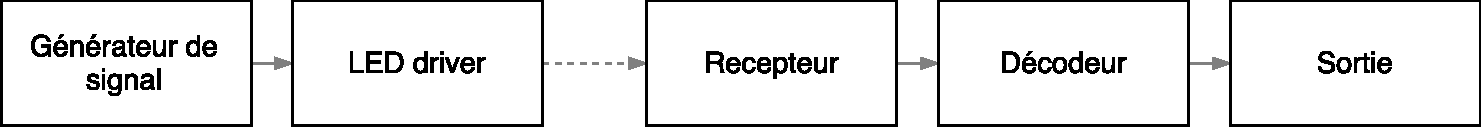
\includegraphics[width=\textwidth]{fig/IRemote_schema_structure}
% \includegraphics[width=0.8\textwidth]{fig/schema_bloc}
\caption{Schéma bloc du système avec signaux}
\label{fig:schema_bloc}
\vspace{5mm}
\end{figure}

Le but de la structure choisie est de faciliter le développement et la testabilité
du sous-système.



%-------------------------------------------------------------------------------
\section{Notation et nomenclature}

\begin{center}
	\begin{tabular}{| c | l | l |}
		\hline
		$n_{pulse}$	& Nombre de pulses dans une salve (addressage) & $13$ \\ \hline
		$t_0$				& Durée high d'un pulse	& $\SI{0.1}{\milli\second}$	\\ \hline
		$T_0$				& Période des pulse	& $\SI{1.0}{\milli\second}$	\\ \hline
		$D_0$				& Duty cycle dans une salve & $10\%$	\\ \hline
		$\tau$			& Période des slaves	& $\SI{0.1}{\second}$\\ \hline
		$t_{miss}$  & &\\ \hline
		$t_{true}$  & Durée du pulse signal une salve correcte & \\ \hline
	\end{tabular}
\end{center}

\begin{center}
    \begin{tabular}{| c | l | c |}
			\hline
        \textit{pulse}      &  \\ \hline
    \end{tabular}
\end{center}
\todo[inline]{TODO: tableau pas fini}

\subsection{Générateur de signal}
Le générateur de signal génère dans OUTPUT des salves de $n_{pulses}$ à une période $\tau$ en active high tant que celui-ci est alimenté à 3V. Les pulses dans les salves ont une durée high $t_0$ et une période $T_0$. Le nombre de pulses et les durées ne sont pas garanties lorsque l'alimentation est retirée.




\begin{description}[leftmargin=!,labelwidth=3cm, labelindent=\parindent]
	\item[Pulse timer] Génère des impulsion à hautes fréquences tant qu'il n'est pas RESET
	\item[Burst timer] Oscille à une période $\tau$ pour signaler le début d'une salve.
	\item[Decounter] Compte le nombre de pulses reçu depuis son dernier RESET et signal lorsque $n_{pulse}$ pulses ont été reçu.
	\item[Logic] Assure les conditions logiques sur les signaux.
\end{description}

\todo[inline]{dimensionnement de valeurs R et C}

\subsection{LED driver}

\subsection{Récepteur et filtrage}

\subsection{Décodeur}
Le décodeur à 3 fonctions:
\begin{itemize}
    \item{Le comptage des pulses assuré par le \emph{decounter}. Celui-ci signal en \emph{active high} si $n_{pulse}$ ont été reçus par la tension d'entrée depuis son dernier \emph{reset}.}
    \item{La détection de pulse manquant assuré par le \emph{missing pulse detector}. Celui-ci signal en \emph{active low} si la tension d'entrée est maintenue \emph{low} pendant au moins $t_{miss} = xxx \si{\milli\second}$ après la fin d'un pulse.}
    \item{La génération du signal sortant assuré par un délais et des portes logiques. Celui si génère en \emph{active high} un pulse de $t_{true} = xx\si{\milli\second}$ si la salve est \emph{correcte}.}
\end{itemize}

Une salve est considéré correcte si le \emph{missing pulse }
\begin{center}
    \begin{tabular}{| m{4cm} | m{4cm} | l | c |}
        \hline
    % \thead{\emph{Missing pulse detector}} & \thead{\emph{Decounter}} & \thead{Statu}} & \thead{Sortie}}\ \hline
    % \thead{\emph{Missing pulse detector}} & \thead{\emph{Decounter}} & \thead{Statu} & \thead{Sortie}\\ \hline
        low     & low       & Nombre incorrect de pulses dans la salve & low \\ \hline
        low     & high  & Salve correcte    & high\\ \hline
        high    & low       & Salve non finie & low \\ \hline
        high    & high  & Salve non finie & low \\ \hline
    \end{tabular}
\end{center}

\subsection{Sortie}

\subsection{Mesures}

\begin{figure}
\begin{minipage}[b]{0.5\linewidth}
\centering
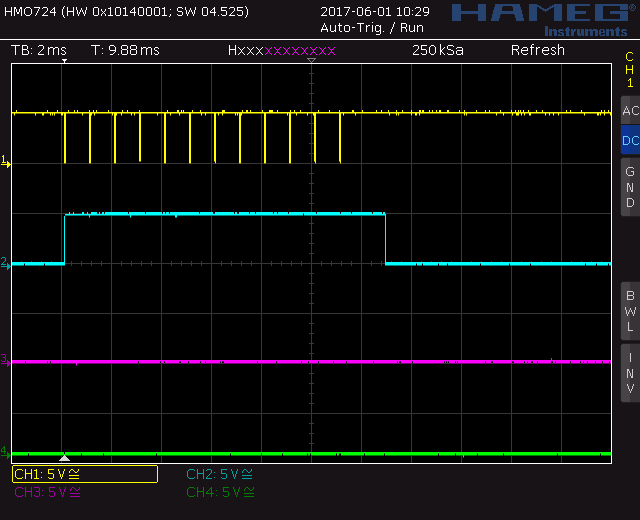
\includegraphics[width=\textwidth]{../measurements/SCR06}
\end{minipage}
\hspace{0.05cm}
\begin{minipage}[b]{0.5\linewidth}
\centering
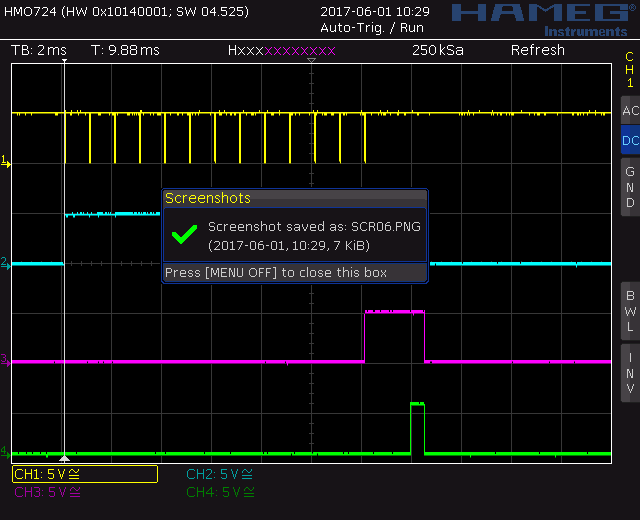
\includegraphics[width=\textwidth]{../measurements/SCR07}
\end{minipage}
\begin{minipage}[b]{0.5\linewidth}
\vspace{0.05cm}
\centering
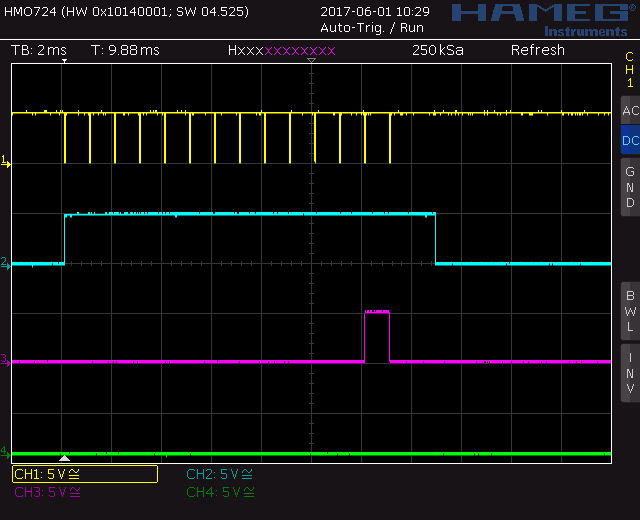
\includegraphics[width=\textwidth]{../measurements/SCR08}
\end{minipage}
\hspace{0.05cm}
\begin{minipage}[b]{0.5\linewidth}
\centering
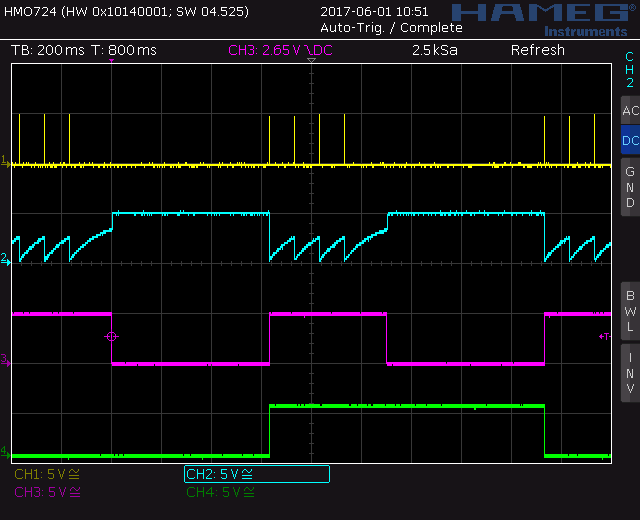
\includegraphics[width=\textwidth]{../measurements/SCR12}
\end{minipage}
\caption{todo}
\end{figure}

\section{Annexes}


\end{document}
